\textbf{See the instruction for questions \inteval{\value{question}+1} to \inteval{\value{question}+2}.}

\begin{figure}[H]
\centering
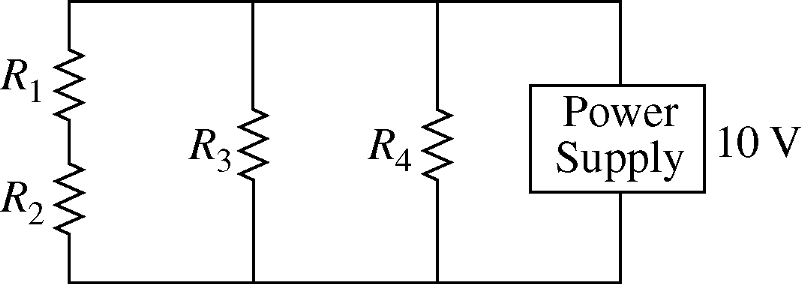
\includegraphics[scale=0.25]{images/img-003-008.png}
\end{figure}

Four resistors, all with the same resistance $R$, are connected as shown above.

% Multiple Choice Question 4
\begin{questions}\setcounter{question}{3}\question
What is the equivalent resistance of the network?

\begin{oneparchoices}
\choice $4 R$
\choice $3 R$
\choice $5 R / 2$
\choice $R$
\choice $2 R / 5$
\end{oneparchoices}\end{questions}

% Multiple Choice Question 5
\begin{questions}\setcounter{question}{4}\question
If the power supply produces $10 \unit{V}$ and the resistance $R$ is $5\latinunit{\Omega}$, what is the current in resistor $R_{4}$ ?

\begin{oneparchoices}
\choice $15    \unit{A}$
\choice $5     \unit{A}$
\choice $2     \unit{A}$
\choice $1 / 2 \unit{A}$
\choice $1 / 5 \unit{A}$
\end{oneparchoices}\end{questions}

